\documentclass[conference]{IEEEtran}
%+++++++++++++++++++++++++++++++++++++++++++
% Added to commands
\input epsf
\usepackage{graphicx}
\usepackage [french]{babel}
\usepackage [utf8]{inputenc}
\usepackage [T1] {fontenc}
\usepackage{float}
\usepackage{amsmath}
%+++++++++++++++++++++++++++++++++++++++++++
% correct bad hyphenation here
\hyphenation{op-tical net-works semi-conduc-tor IEEEtran}
\begin{document}

%+++++++++++++++++++++++++++++++++++++++++++
\title{\LARGE L'équilibre d'un kite
\vskip10pt

\small 2024 - Romain LAMBERT
}
%+++++++++++++++++++++++++++++++++++++++++++
% make the title area
\maketitle

\begin{abstract}Ce bureau d'étude a pour sujet l'équilibre du Kite, sa condition d'existence et sa stabilité. L'objectif final étant de déterminer des paramètres optimaux tels que le towpoint. 
\end{abstract}
\IEEEoverridecommandlockouts

\IEEEpeerreviewmaketitle
\section{L'équilibre du kite}

\subsection{$X_T$} 

le point d'application d'un effort est une notion importante. Si celui de l'effort aérodynamique et du poids sont couramment utilisés, le point d'application de la tension des lignes influence beaucoup les performances d'un kite. De plus, le bridage d'un kite change considérablement la façon dont se répartie la tension dans les lignes et l'angle d'équilibre au zénith d'un kite. Ainsi, afin de capturer l'influence du bridage sur les performances d'un kite, on définit $X_T$ comme étant \textbf{le point d'intersection entre la corde moyenne d'un kite et l'axe de la tension des lignes}. Ainsi, $X_T$ permet de lié la géométrie du bridage et son influence sur la dynamique du kite.  \\

\begin{figure}[H]
    \centering
    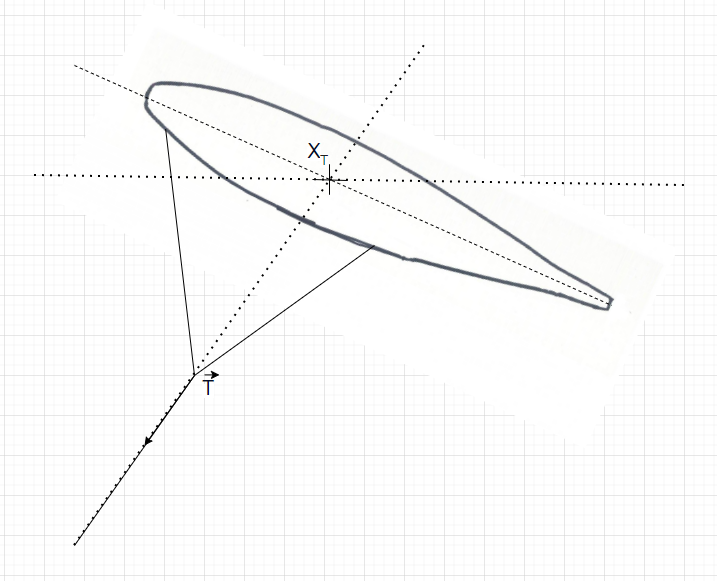
\includegraphics[width=0.5\textwidth]{Pics/Xt.png}  
    \caption{Xt}
    \label{fig:Xt}
\end{figure}

Isoler les ensembles \{kite\} et \{kite+bridage\} permet de montrer $X_T$ est le point d'application de l'ensemble du bridage, le long de la corde. En effet :

Pour l'équilibre des moments appliqué à l'ensemble \{kite\}, en le $X_T$ :
\begin{equation}
    F_{Poid}(x_G-x_{TP})+F{aero}(x_{aero}-x_{TP}) = 0
\end{equation}

Pour l'équilibre des moments appliqué à l'ensemble \{kite+bridage\}, $X_T$:
\begin{equation}
    F_{Poid}(x_G-x_{TP}) + F{aero}(x_{aero}-x_{TP}) + \sum_{i=A}^{D} F_{ligne i}(x_{ligne i}-x_{TP})= 0
\end{equation}

D'où : 
\begin{equation}
    \sum_{i=A}^{D} F_{ligne i}(x_{ligne i}-x_{TP})= 0
\end{equation}

Ce qui, par définition, montre que \textbf{$X_T$ est le point d'application de la résultante de tension de l'ensemble du bridage projeté sur la corde.}

\subsection{l'Equilibre} 

\begin{figure}[H]
    \centering
    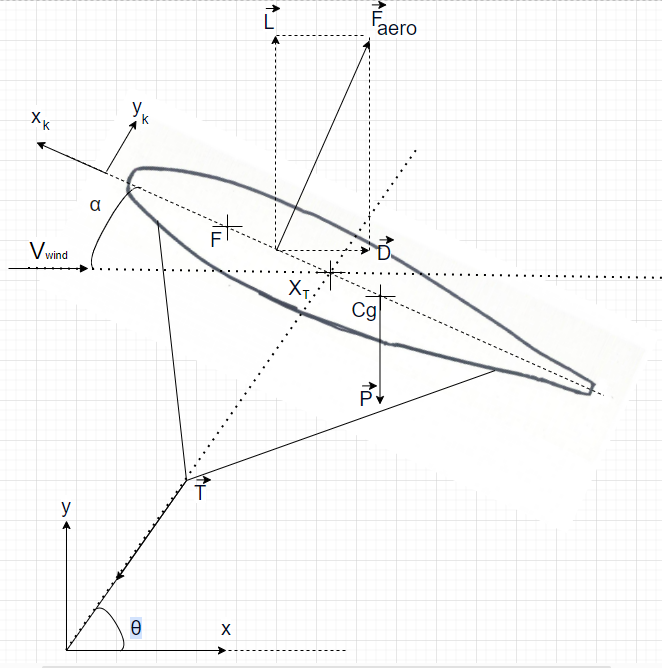
\includegraphics[width=0.5\textwidth]{Pics/Equilibre Kite.png}  
    \caption{Equilibre du kite}
    \label{fig:Equilibre du kite}
\end{figure}

On écrit l'équilibre statique de \{kite+bridage\}, en $X_T$ du kite : 

\begin{equation}
    \begin{cases}
        L = P + T sin(\theta) \\
        D = T cos(\theta) \\
        0 = C_{M_0} + (x_{TP} - x_F) (L cos(\alpha) + D sin(\alpha)) - P cos(\alpha) (x_{TP} - x_G)
    \end{cases}
\end{equation}

Ainsi, en considérant $\alpha << 1$, on a :

\begin{equation}
    \begin{cases}
    \frac{L-P}{D} = tan(\theta) \\
    \theta = \alpha + \alpha_0 \\
    x_{TP} = \frac{L x_F - P x_G -C_{M_0}}{L - P}
    \end{cases}
    \label{eq:Xtp}
\end{equation}
    
Il semblerait donc que le calcul (CFD, VSM, ...) des polaires aérodynamiques ($L(\alpha)$ et $D(\alpha)$) permettent de trouver le $X_T$ optimal afin d'optimiser la finesse au zénith. 

\textit{Exemple : }
Pour $\alpha_{optimal} = 21^\circ$, $C_D = 0.19$ et $C_L = 1.35$, on trouve en appliquant l'équation \ref{eq:Xtp} : \\

\begin{equation}
    \begin{cases}
    \alpha_0 =  -12^\circ\\
    \theta = 9^\circ\\
    x_{TP} = 0.22
    \end{cases}
    \label{eq:Xtp}
\end{equation}

avec $P = 21 kg$, $x_F = 0.25$, $x_G = 0.5$,$\frac{1}{2} \rho S v^2 = \frac{1}{2} 1.225 * (50m^2) * (14 * 0.514 m/s)^2$  et $C_{M_0} = 0$

\IEEEpeerreviewmaketitle
\section{Condition d'existence de l'équilibre du kite }

\subsection{Angle d'élévation minimal} 


\subsection{Angle d'élévation maximal}

\section{Stabilité du kite }

\end{document}